% vim: tw=78:ts=2:sw=2:et:fdm=marker:wrap
\def\TITLE{Mobil po\"{a}ngb\"{o}rsapplikation med databaskoppling via
webbtj\"{a}nst}
\def\AUTHOR{Oskar Sch\"{o}ldstr\"{o}m \& Alex Fagerstr\"{o}m}

\documentclass[swedish,a4paper]{article}

\usepackage[left=2cm,top=2cm,right=2cm,bottom=2cm]{geometry}
\usepackage[utf8]{inputenc}
\usepackage[T1]{fontenc}
\usepackage[swedish]{babel}
\usepackage[pdftex]{hyperref} % Hyperlinks
\usepackage{graphicx}
\usepackage{cancel}
\usepackage{setspace}
\usepackage{array}

\hypersetup{pdftitle={\TITLE}}
\hypersetup{pdfauthor={\AUTHOR}}
\hypersetup{pdfkeywords={}}
\hypersetup{pdfsubject={\TITLE}}
\hypersetup{colorlinks}
\setcounter{secnumdepth}{-1}

\title{\TITLE}
\author{\AUTHOR}

\pagestyle{myheadings}
\markright{Fortsättningskurs i datanät (2012-2013)}

\begin{document}

\maketitle

\section{Projekt}

\textbf{Avklarade delmoment:} 6 \\

\subsubsection{Delmoment}
\begin{enumerate}
  \item Denna uppgift gjordes inte eftersom den uppfyldes senare, RCP
    backenden är implementerad i Node.js med hjälp av bl.a. Restify
    biblioteket.
  \item Även denna uppgt skippades eftersom det implementeras senare.
    RCP funktionen är implementerad sedan punkt 1.
  \item Finns en restify route som tar emot en lista av player objekt.
    Attributen goals samt assists adderas till spelarens tidigare
    statistik och dess game counter inkrementeras.
  \item MongoDB och dess nodejs bibliotek Mongoose används.
    Implementerades redan iom. punkt 1.
  \item Inloggningen sker mha. HTTP Basic Authentication som måste följa
    med varje request till backenden. SSL fixat mha. ett litet bash
    script vi skrivit för att underlätta framtida arbete.
    \begin{itemize}
      \item Filerna genereras med att köra ./build/cert.sh
    \end{itemize}
  \item Eftersom den distribuerade MongoDB native driver inte har SSL
    stöd och skulle kräva en omkompilering kan vi inte visa upp detta
    iom.  att web servicen är hostad på en development server i bruk.
    Dock fungerar det om man kompilerar MongoDB med SSL och
    avkommenterar SSL raderna i config.js. Konfigurationer bör göras i
    \textit{/etc/mongodb.conf}
    \begin{itemize}
      \item \textit{bind\_ip} måste kommenteras bort för att lyssna på annat än
        loopback
      \item \textit{port} bör vara 27017 för att överensstämma med
        \textit{config.js}
      \item \textit{auth} bör vara true samt man bör skapa en user via
        mongo localhost klienten.
      \item \textit{sslOnNormalPorts = true\\
        sslPemKeyFile = ./cert/mongodb/mongodb.pem\\
        sslPemPassword = pass}
    \end{itemize}
\end{enumerate}

\section{Klassdiagram}

\textbf{Skissera upp ett klassdiagram över din/er applikation på serversidan och
beskriv kort rollen av varje klass. Beskriv även klasstrukturen på klientsidan
om den modifierats från den ursprungliga.}
\\
\\
Det existerar även dokumentation i formen av test generated docs och annotated
source. Se docs/index.html eller
\url{http://innebandy.oxy.minas-tirith.genero.fi/docs/}

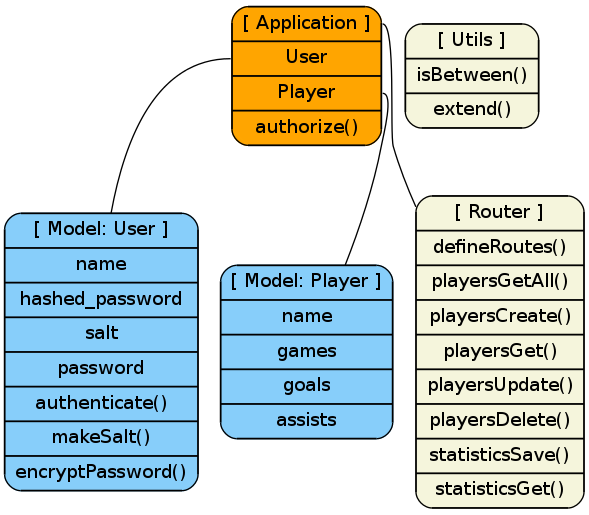
\includegraphics[width=12cm]{../dot/class.png}

\end{document}
